%!TEX root = ../../thesis.tex

\section{Timing}
\label{sec:webaudio-timing}

\begin{quote}
  ``Silence is very important. The silence between the notes is as important as the notes themselves.'' - Wolfgang Amadeus Mozart
\end{quote}

One of the most important aspects of making music, no matter if it's digital or analogue, is timing. Songs are made of notes which are played at specific points in time. The gaps between the notes create a rhythm which plays a big role in the perception of songs. Only knowing about the individual notes of a composition is useless without having information about the rhythm and, therefore, about the timing.

\subsection{Timing methods in JavaScript}
\label{subsec:timing-in-js}

In JavaScript there are several ways to time code execution. The global method \code{setTimeout(func, delay)} \cite[chapter: setTimeout]{MDN} delays the execution of \code{func} by \code{delay} milliseconds. So, if an arbitrary function called \code{doIt} should be executed after one second, the code would look like this: \code{setTimeout(doIt, 1000)}. The execution of \code{func} can be prevented by calling \code{clearTimeout(timeoutId)} with the id that was returned by \code{setTimeout}.

Besides \code{setTimeout} there is also \code{setInterval(func, delay)} \cite[chapter: setInterval]{MDN} which will repeatedly execute \code{func} each time \code{delay} milliseconds have passed. In line with the above mentioned \code{clearTimeout\allowbreak (timeoutId)}, the execution of \code{func} can be prevented by calling \code{clearInterval\allowbreak (intervalId)}.

In theory, these methods could be used to properly time sounds and arrangements but they have some drawbacks. The JavaScript runtime does not guarantee that callbacks are called exactly at the specified point in time. Generally, the execution is off from the planned point in time by some milliseconds, even when there are no heavy computations on the website\footnote{\url{http://jsfiddle.net/janmonschke/sar5x/}, last checked on 10/03/2014}. The delay can even increase by several hundred milliseconds when there is user interaction like a window resize or a tab switch. In most browsers, interval times are also limited when the current tab becomes inactive. The Mozilla documentation states that in their implementation ``intervals are clamped to fire no more often than once per second in inactive tabs''\footnote{\cite[chapter: setInterval]{MDN}}. All these problems make the methods useless for the needs of precise audio timing. 

\subsection{Timing nodes in the Web Audio API}
\label{subsec:timing-in-web-audio}

Timing in the Web Audio API does not rely on any of the normal JavaScript timing methods. Each \code{AudioContext} has a \code{currentTime} property which returns the precise amount of seconds that have passed since the context has been created. This property can be used to time the beginning of a buffer or the beginning of an oscillator. As described in \refchapter{sec:webaudio-buffer}, buffers are started by calling their \code{start} method. The buffer's \code{start} method has three parameters: \code{buffer.start(when, offset, duration)}. \code{when} defines the point in time at which the buffer should be started, \code{offset} defines the amount of seconds that should be skipped and \code{duration} defines for how long the buffer should be played. The unit for all these values, as well as for all other values in the Web Audio API that deal with timing, is seconds. The oscillator's (\refchapter{sec:webaudio-osc}) \code{start} method only has a \code{when} parameter because \code{offset} and \code{duration} only make sense for nodes with a predefined length.

\begin{lstlisting}[language=JavaScript, caption=Usage of the start method's parameters, label=lst:currentTime]
  buffer.start(context.currentTime + 1, 2, 1);

  oscillator.start(context.currentTime + 1)
\end{lstlisting}

\reflisting{lst:currentTime} illustrates how to use \code{context.currentTime} in combination with the \code{start} method. Line 1 schedules a buffer to start in one second with a buffer-offset of two seconds and will end the playback after a duration of one second. Line 2 starts an oscillator in one second. It is important, that the \code{currentTime} is added to the \code{when} parameter, because the Web Audio API starts nodes by comparing the \code{when} parameter to \code{currentTime}. If only \code{1} were passed as the first parameter in line 1, it would not get scheduled to play in one second but at whatever point in time is defined by \code{currentTime - 1}.

To demonstrate how powerful the \code{start} method is, the following listings will show how to write a simple drum loop and a scheduler that only uses the \code{when} parameter.

A drum loop is a series of beats of which each represents an individual percussion instrument that is typically found in drum sets, such as a snare drum or a kick drum. The example loop has sixteen beats and consists of three different sounds (`hihat', `kick', `snare'). Scheduling the drum loop can be done with only a for-loop that iterates over the amount of beats. \reflisting{lst:drumloop} schedules a simple drum pattern that plays the hihat on every other odd beat, it plays the kick drum on beats one and nine and it plays the snare drum on beats five and thirteen.

\begin{lstlisting}[language=JavaScript, caption=Scheduling a simple drum loop, label=lst:drumloop]
  for(var i = 1; i < 17; i++){
    if(i % 2 == 1)
      play("hihat", i);

    if(i == 1 || i == 9)
      play("kick", i);

    if(i == 5 || i == 13)
      play("snare", i);
  }
\end{lstlisting}

The above example lacks some information on how the scheduling actually works. So far it only contains details about which note to play on which beat but no details about the speed, which is, as already described above, necessary to perform, or in this case to schedule, the song.

The speed of a song is often described in \emph{beats per minute (bpm)}. The \code{play} method in the next example only needs to know about the seconds between each beat to properly schedule a beat. As \reflisting{lst:rhythmscheduling} shows in line six, the scheduling of a sound is done by simply multiplying the index of its beat by \code{secondsBetweenBeats} which is calculated in line three from the \code{bpm} and the speed\footnote{Dividing (60 / bpm) by 4 creates the time in seconds between 16th notes.}.

\begin{lstlisting}[language=JavaScript, caption=Scheduling with a certain speed, label=lst:rhythmscheduling]
  var bpm = 120;
  var secondsBetweenBeats = (60 / bpm) / 4;

  var play = function(buffer, beat){
    var bufferNode = getBuffer(buffer);
    bufferNode.start(beat * secondsBetweenBeats);
  };
\end{lstlisting}

Of course, this scheduler is very limited because it is only capable of playing a drum loop once and there is no way to change the speed or the rhythm, but it is a good example that shows how a basic, precise scheduler can be implemented. \refchapter{sec:impl-scheduling} introduces a more complex and feature-rich scheduler that makes use of old (\code{window.setInterval}) and new (\code{node.start}) timing methods in combination.

\subsection{Timing parameters}

The Web Audio API also gives fine grained access to a node's parameters and allows for the ability to time and to interpolate them in various ways. Parameter values, however, cannot be changed directly but have to be changed by accessing a parameters's \code{value} property like so: \code{gn.gain.value = 1.2}. By using the GainNode's \code{setValueAtTime} method, this operation can be scheduled to a point in the future, e.g. \code{gn.gain.setValueAtTime(2, now + 1)} (assuming that \code{now = context.currentTime}) will set the gain to the value of two in one second from now.

In addition to that, a node's parameters can also be interpolated over time by using their \code{linearRampToValueAtTime} method: \code{linearRampToValueAtTime (2, now + 2)} will interpolate the gain's value linearly for two seconds, until it has reached the value of two. Nodes also have methods to interpolate parameters exponentially (\code{exponentialRampToValueAtTime}) and to interpolate parameters using a custom curve (\code{setValueCurveAtTime}) and their description can be found in the official Web Audio documentation\footnote{\url{http://webaudio.github.io/web-audio-api}, accessed 13.03.2014}.

These timing methods are all part of the \code{AudioParam} interface, which is used for all audio parameters, e.g., the oscillator's \code{frequency} parameter, the filter's \code{Q} parameter or the B\code{ufferSourceNode's playbackRate}. They make it much easier and much more accurate to control a node's behavior than it would be by using custom \code{window.setTimeout} handlers.

\subsection{ADSR Envelope}
\label{sec:adsr-envelope}

A perfect use case for parameter timing is the implementation of ADSR envelopes. ADSR is an acronym and stands for Attack, Decay, Sustain and Release envelope. It is a way of controlling the perception of a sound by dividing it into different phases which each have a different amplitude \cite[p. 97]{curtis1996computer}. When artists play a note on a piano, they have full control over how hard they push a key and therefore control over the attack of a sound, which, depending on the power that is used, can be louder than the rest of the sound. This effect cannot be reproduced with normal (digital) computer keyboards, because they can only be pressed or released. These keyboards can mimic the length of a sound. It might sound like a slight detail to influence the sound with ADSR envelopes, but it is actually a very common way to compose unique and distinguishable sounds.

\begin{figure}[htb]
  \centerline{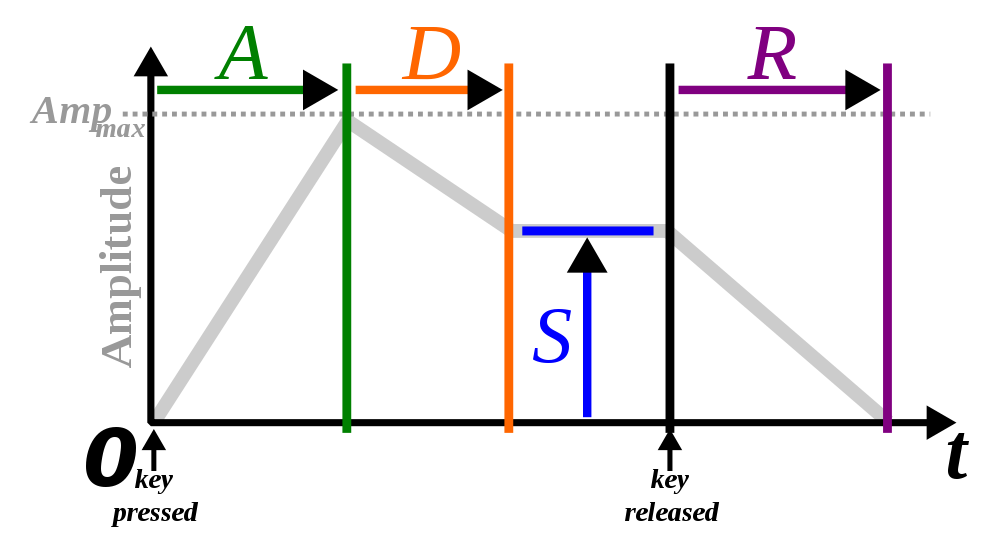
\includegraphics[width=0.8\linewidth]{images/ADSR_parameter.png}}
  \caption[Impact of an ADSR envelope on a sound's amplitude over time -
  \protect\newline{\small\url{http://commons.wikimedia.org/wiki/File:ADSR_parameter.svg} (01.23.2014)}
  \protect\newline{\small\emph{WikiMedia - User:Abdull}}]{Impact of an ADSR envelope on a sound's amplitude over time}
  \label{fig:ADSR}
\end{figure}

\reffigure{fig:ADSR} shows the four different phases of an ADSR envelope.

\begin{description}
  \item[Attack] \hfill \\
  The time it takes to reach the max level, starting from zero when the key is pressed.
  \item[Decay] \hfill \\
  The time it takes to interpolate to the sustain level.
  \item[Sustain] \hfill \\
  The normal amplitude level of the sound. Depending on the application, sustain either can be defined only as an amplitude level or the sustain property of an envelope can also contain duration information.
  \item[Release] \hfill \\
  Interpolation time to zero, starting from the sustain level when the key is released.
\end{description}

This concept gives us the option to control a sound like piano players (the piano pedal information is based on: \cite[p. 72]{pilhofer2011music}). The attack and the decay parameters correlate to the key pressure and the key speed. A shorter attack value leads to a sharper sound, whereas a longer attack value makes a sound softer. The sustain parameter, if it contains a duration information, is similar to the effect that is created by using the sostenuto pedal on a piano (middle pedal), it will sustain the sound until the pedal is released. Release time can be altered by using the damper pedal (right pedal), which will release the dampers and make the tones sound longer.

\begin{lstlisting}[language=JavaScript, caption=A minimalistic ADSR envelope in JavaScript, label=lst:adsrenvelope]
  var keydown = function(){
    var now = context.currentTime;
    buffer.gain.setValueAtTime(0, now);
    buffer.gain.linearRampToValueAtTime(maxLevel, now + attack); // ATTACK
    buffer.gain.linearRampToValueAtTime(sustainLevel, now + attack + decay ); // DECAY
  };

  var keyup = function(){
    var now = context.currentTime;
    buffer.gain.value.linearRampToValueAtTime(0, now + release); // RELEASE
  };

  document.addEventListener("keydown", keydown);
  document.addEventListener("keyup", keyup);
\end{lstlisting}

In \reflisting{lst:adsrenvelope}, a minimal envelope is implemented using the above mentioned timing methods. It assumes that \code{buffer} is a \code{BufferSourceNode} which is already loaded, that \code{context} is a \code{WebAudioContext} and that \code{maxLevel} and \code{sustainLevel} are predefined number values. The methods \code{keydown} and \code{keyup} are executed whenever their corresponding events are fired on the \code{document} object (lines 13--14). In \code{keydown}, the buffer's gain is set to zero initially (line 3) and then scheduled to rise up to the \code{maxLevel} value after the \code{attack} time has passed (line 4). Directly after that, the gain is scheduled to go down to the \code{sustainLevel} after the decay time has passed (line 5). On first sight, it might look wrong to schedule two linear interpolations at the same time, because they would interfere with each other if they were run simultaneously. In the Web Audio API, however, all scheduling methods are executed consecutively for each parameter so that two scheduled events on the same parameter cannot interfere \cite[Chapter 4.5.2.]{wilson2014webaudiospec}. In the example above, it means that the decay-interpolation is not triggered until the attack-interpolation finished. When a key on the keyboard is released, the \code{keyup} handler will interpolate the buffer's gain to zero for as long as \code{release} was set (line 10). 